\documentclass[aspectratio=169,10pt]{beamer}
\usepackage[utf8]{inputenc}
\usepackage[T1]{fontenc}
\usepackage{amsmath,amsfonts,amssymb}
\usepackage{graphicx}
\usepackage{xcolor}
\usepackage{tikz}
\usetikzlibrary{shapes,arrows.meta,positioning,fit,calc,shadows}
\usepackage{booktabs}
\usepackage{array}
\usepackage{colortbl}
\usepackage{listings}
\usepackage{hyperref}

\usetheme{Madrid}
\usecolortheme{default}
\setbeamertemplate{navigation symbols}{}
\setbeamertemplate{footline}[frame number]

\AtBeginSection[]{}
\AtBeginSubsection[]{}

\definecolor{mlblue}{RGB}{0,102,204}
\definecolor{mlgreen}{RGB}{0,153,76}
\definecolor{mlorange}{RGB}{255,102,0}
\definecolor{mlred}{RGB}{204,0,51}
\definecolor{mlpurple}{RGB}{102,51,153}
\definecolor{codebg}{RGB}{245,245,248}

\setbeamercolor{structure}{fg=mlblue}
\setbeamercolor{block title}{bg=mlblue,fg=white}
\setbeamercolor{block body}{bg=mlblue!8}
\setbeamercolor{alerted text}{fg=mlred}
\setbeamercolor{example text}{fg=mlgreen}

\lstdefinestyle{pythonstyle}{
    language=Python,
    basicstyle=\ttfamily\scriptsize,
    keywordstyle=\color{mlblue}\bfseries,
    commentstyle=\color{mlgreen!70!black}\itshape,
    stringstyle=\color{mlred},
    showstringspaces=false,
    breaklines=true,
    frame=single,
    rulecolor=\color{gray!40},
    backgroundcolor=\color{codebg},
    numbers=left,
    numberstyle=\tiny\color{gray},
    numbersep=4pt,
    xleftmargin=1.2em
}
\lstset{style=pythonstyle}

\title[HTTP \& REST]{HTTP \& REST Fundamentals}
\subtitle{Topic 1: The foundation of every API}
\author{ML + UI + API + MCP Project}
\institute{Learning Path}
\date{\today}

\begin{document}

\begin{frame}
\titlepage
\end{frame}

\begin{frame}{Outline}
\tableofcontents
\end{frame}

\section{Why HTTP and REST?}

\begin{frame}{Why start here?}
\begin{block}{Key idea}
Every API call, UI request, and MCP tool wrapper you will build rides on top of HTTP.
\end{block}
\begin{columns}[T]
\begin{column}{0.48\textwidth}
\begin{itemize}
\item \textbf{HTTP}: the protocol clients and servers use to talk.
\item \textbf{REST}: a style for designing APIs around resources.
\item \textbf{JSON}: the common data format in the body.
\end{itemize}
\end{column}
\begin{column}{0.48\textwidth}
\begin{alertblock}{ML application}
Your linear regression model will live behind a \texttt{POST /predict} endpoint: the UI sends features, the API returns a prediction.
\end{alertblock}
\end{column}
\end{columns}
\end{frame}

\section{Request and Response}

\begin{frame}{The client--server cycle}
\begin{center}
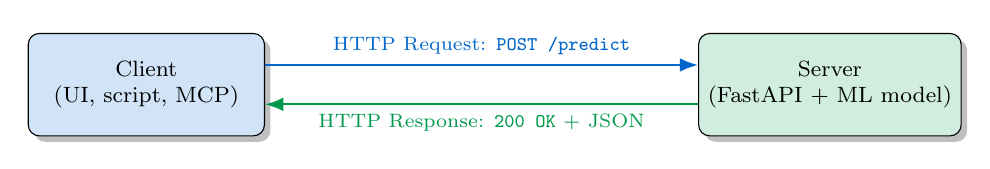
\begin{tikzpicture}[
  box/.style={draw, rounded corners, align=center, minimum height=1.3cm,
              minimum width=3cm, font=\footnotesize, drop shadow},
  arr/.style={-{Latex}, thick}
]
  \node[box, fill=mlblue!18] (c) {Client\\(UI, script, MCP)};
  \node[box, fill=mlgreen!18, right=5.5cm of c] (s) {Server\\(FastAPI + ML model)};
  \draw[arr, mlblue] ([yshift=0.25cm]c.east) -- node[above, font=\scriptsize]
    {HTTP Request: \texttt{POST /predict}} ([yshift=0.25cm]s.west);
  \draw[arr, mlgreen] ([yshift=-0.25cm]s.west) -- node[below, font=\scriptsize]
    {HTTP Response: \texttt{200 OK} + JSON} ([yshift=-0.25cm]c.east);
\end{tikzpicture}
\end{center}
\vspace{0.3cm}
\begin{block}{Stateless}
Each request carries everything the server needs; the server keeps no memory between calls.
\end{block}
\end{frame}

\begin{frame}{Anatomy of a request and a response}
\begin{columns}[T]
\begin{column}{0.48\textwidth}
\begin{exampleblock}{Request}
\begin{itemize}
\item \textbf{Method}: what to do
\item \textbf{URL}: which resource
\item \textbf{Headers}: metadata (\texttt{Content-Type})
\item \textbf{Body}: data (JSON)
\end{itemize}
\end{exampleblock}
\end{column}
\begin{column}{0.48\textwidth}
\begin{exampleblock}{Response}
\begin{itemize}
\item \textbf{Status code}: result of the call
\item \textbf{Headers}: metadata
\item \textbf{Body}: returned data (JSON)
\end{itemize}
\end{exampleblock}
\end{column}
\end{columns}
\end{frame}

\section{Methods and Status Codes}

\begin{frame}{HTTP methods (CRUD)}
\begin{center}
\begin{tabular}{llll}
\toprule
\textbf{Method} & \textbf{Action} & \textbf{Example} & \textbf{Safe?} \\
\midrule
\texttt{GET}    & Read    & \texttt{GET /models}       & Yes \\
\texttt{POST}   & Create / run & \texttt{POST /predict} & No \\
\texttt{PUT}    & Replace & \texttt{PUT /models/1}     & No \\
\texttt{PATCH}  & Update part & \texttt{PATCH /models/1} & No \\
\texttt{DELETE} & Remove  & \texttt{DELETE /models/1}  & No \\
\bottomrule
\end{tabular}
\end{center}
\begin{alertblock}{ML application}
Predictions use \texttt{POST} because features travel in the body, not the URL.
\end{alertblock}
\end{frame}

\begin{frame}{Status codes}
\begin{center}
\begin{tabular}{lll}
\toprule
\textbf{Range} & \textbf{Meaning} & \textbf{Common codes} \\
\midrule
\rowcolor{mlgreen!12} 2xx & Success & 200 OK, 201 Created \\
\rowcolor{mlblue!10}  3xx & Redirect & 301, 304 \\
\rowcolor{mlorange!15} 4xx & Client error & 400, 401, 404, 422 \\
\rowcolor{mlred!12}   5xx & Server error & 500, 503 \\
\bottomrule
\end{tabular}
\end{center}
\begin{block}{Remember}
\texttt{422} = valid JSON but wrong fields (e.g.\ text instead of a number); \texttt{500} = your server code failed.
\end{block}
\end{frame}

\section{JSON and Example}

\begin{frame}[fragile]{JSON payloads for a prediction}
\begin{columns}[T]
\begin{column}{0.48\textwidth}
\textbf{Request body}
\begin{lstlisting}[numbers=none]
POST /predict
Content-Type: application/json

{
  "square_feet": 1850,
  "bedrooms": 3
}
\end{lstlisting}
\end{column}
\begin{column}{0.48\textwidth}
\textbf{Response body}
\begin{lstlisting}[numbers=none]
HTTP/1.1 200 OK
Content-Type: application/json

{
  "predicted_price": 412500.0
}
\end{lstlisting}
\end{column}
\end{columns}
\end{frame}

\begin{frame}[fragile]{Calling an API from Python}
\begin{lstlisting}
import requests

url = "http://127.0.0.1:8000/predict"
payload = {"square_feet": 1850, "bedrooms": 3}

response = requests.post(url, json=payload, timeout=10)
print(response.status_code)   # 200
print(response.json())        # {'predicted_price': 412500.0}
\end{lstlisting}
\end{frame}

\section{REST Principles}

\begin{frame}{REST principles at a glance}
\begin{columns}[T]
\begin{column}{0.48\textwidth}
\begin{itemize}
\item \textbf{Resources}: nouns in URLs (\texttt{/models}), not verbs.
\item \textbf{Stateless}: no session memory on the server.
\item \textbf{Uniform interface}: standard methods and status codes.
\end{itemize}
\end{column}
\begin{column}{0.48\textwidth}
\begin{itemize}
\item \textbf{Representations}: resources exchanged as JSON.
\item \textbf{Client--server}: UI and backend evolve independently.
\item \textbf{Cacheable}: \texttt{GET} responses can be reused.
\end{itemize}
\end{column}
\end{columns}
\end{frame}

\section{Takeaways}

\begin{frame}{Takeaways}
\begin{enumerate}
\item HTTP is a request/response conversation between client and server.
\item Choose the method by intent: \texttt{GET} reads, \texttt{POST} sends data.
\item Status codes tell the client what happened (2xx, 4xx, 5xx).
\item JSON is the shared language between UI, API, and MCP.
\item Next topic: \textbf{API Design Principles}.
\end{enumerate}
\end{frame}

\end{document}
